%\section{***Linear Regression Analysis under Sets of Conjugate Priors}
%\label{sec:isipta07}

%***short summary of ISIPTA'07 paper??***


\section{A Parameter Set Shape for Strong Prior-Data Agreement Modelling}
\label{sec:boatshape}

%march 2013 notes (technical results)
%Preliminary results
In this section, we will explain an approach for parameter set shapes
that allow for extra precision in case of strong prior-data agreement
as discussed in Section~\ref{sec:concluding-outlook}.
First, we will briefly characterise the novel parametrisation of canoncial conjugate priors this approach relies on.
To keep things simple, we restrict ourselves here for the case of the Beta-Binomial model
(see Section~\ref{sec:beta-binom}),
but the approach is generalisable to arbitrary canonical conjugate priors.%
\footnote{For a more detailed derivation of this parametrisation,
we have to refer to a future publication of Mi\c{k}elis Bickis.}
Then we will suggest a shape in this parametrisation that accomplishes
both \pdc\ sensitivity and `bonus precision' in case of strong prior-data agreement.
We present a parametric description for such a shape
and show that it will indeed lead to the desired properties.

\subsection{A Novel Parametrisation of Canonical Conjugate Priors}
\label{sec:miksworld}

In the parametrisation in terms of $\nz$ and $\yz$, described in Section~\ref{sec:regularconjugates},
a conjugate priors is updated to its respective posterior by a shift in the parameter space,
given by \eqref{eq:canonicalupdate}:
\begin{align*}
\nz &\mapsto \nz + n\,, &
\yz &\mapsto \frac{\nz}{\nz + n} \cdot \yz + \frac{n}{\nz + n} \cdot \frac{\tau(\x)}{n} = \yz + \frac{\tau(\x)-n\yz}{\nz+n}\,.
\end{align*}
We see thus that, while the shift for the $n$ coordinate is the same for all elements $(\nz,\yz)$
in a prior parameter set $\PZ$,
the shift in the $y$ coordinate depends on $\nz$, and the location of $\yz$ itself.
Due to this, the shape of $\PZ$ will change during the update step.

This shape change makes it very difficult to understand the posterior inference properties
of a certain shape of the prior parameter set $\PZ$.
Therefore, a different parametrisation of the canonical priors
in which each coordinate has the same shift in updating would be advantageous.
Then, updating of parameter sets
could be expressed as a shift of the entire set within the parameter space.
%Although interpretation of the shapes may be slightly more difficult due to the,

A parametrisation developed by Mi\c{k}elis Bickis (personal communication) attains*** just that.
He is currently preparing a manuscript elaborating the details of his findings,
and we will present here a preview on the results for the Beta-Binomial case.

In this parametrisation, a canonical prior is represented by a coordinate $(\eta_0,\eta_1)$,
where $\eta_1$ replaces the main prior parameter $\yz$,
while $\eta_0$ is just a different name for $\nz$.
The relation of $(\eta_0,\eta_1)$ to $(\nz, \yz)$ is as follows:
%\begin{equation}
\begin{align}
\label{eq:trafotony}
%\begin{aligned}
\nz &= \eta_0 \,, &
\yz &= \frac{\eta_1}{\eta_0 + 2} + \frac{1}{2}\,.
%\end{aligned}
%\end{equation}
\end{align}

The domain of $\eta_0$ and $\eta_1$ in case of the Beta-Binomial model is
\begin{align}
\label{eq:eta-domain}
\Eta &= \Big\{ (\eta_0,\eta_1) \Big| \eta_0 > -2,\ |\eta_1| < \frac{1}{2}(\eta_0 + 2) \Big.\Big\}\,,
\end{align}

and the update step in terms of $\eta_0$ and $\eta_1$ is given by
\begin{equation}
\label{eq:eta-update}
\begin{aligned}
\eta_0\un &= \eta_0\uz + n\,, \\
\eta_1\un &= \eta_1\uz + \frac{1}{2}(s - (n-s)) = \eta_1\uz + s - \frac{n}{2}\,,
\end{aligned}
\end{equation}
where we denote prior parameters with suprscript ${}\uz$, and posterior parameters with ${}\un$,
while $s$ is the number of successes in the $n$ Bernoulli trials.

\begin{figure}  %trim=l b r t
\centering
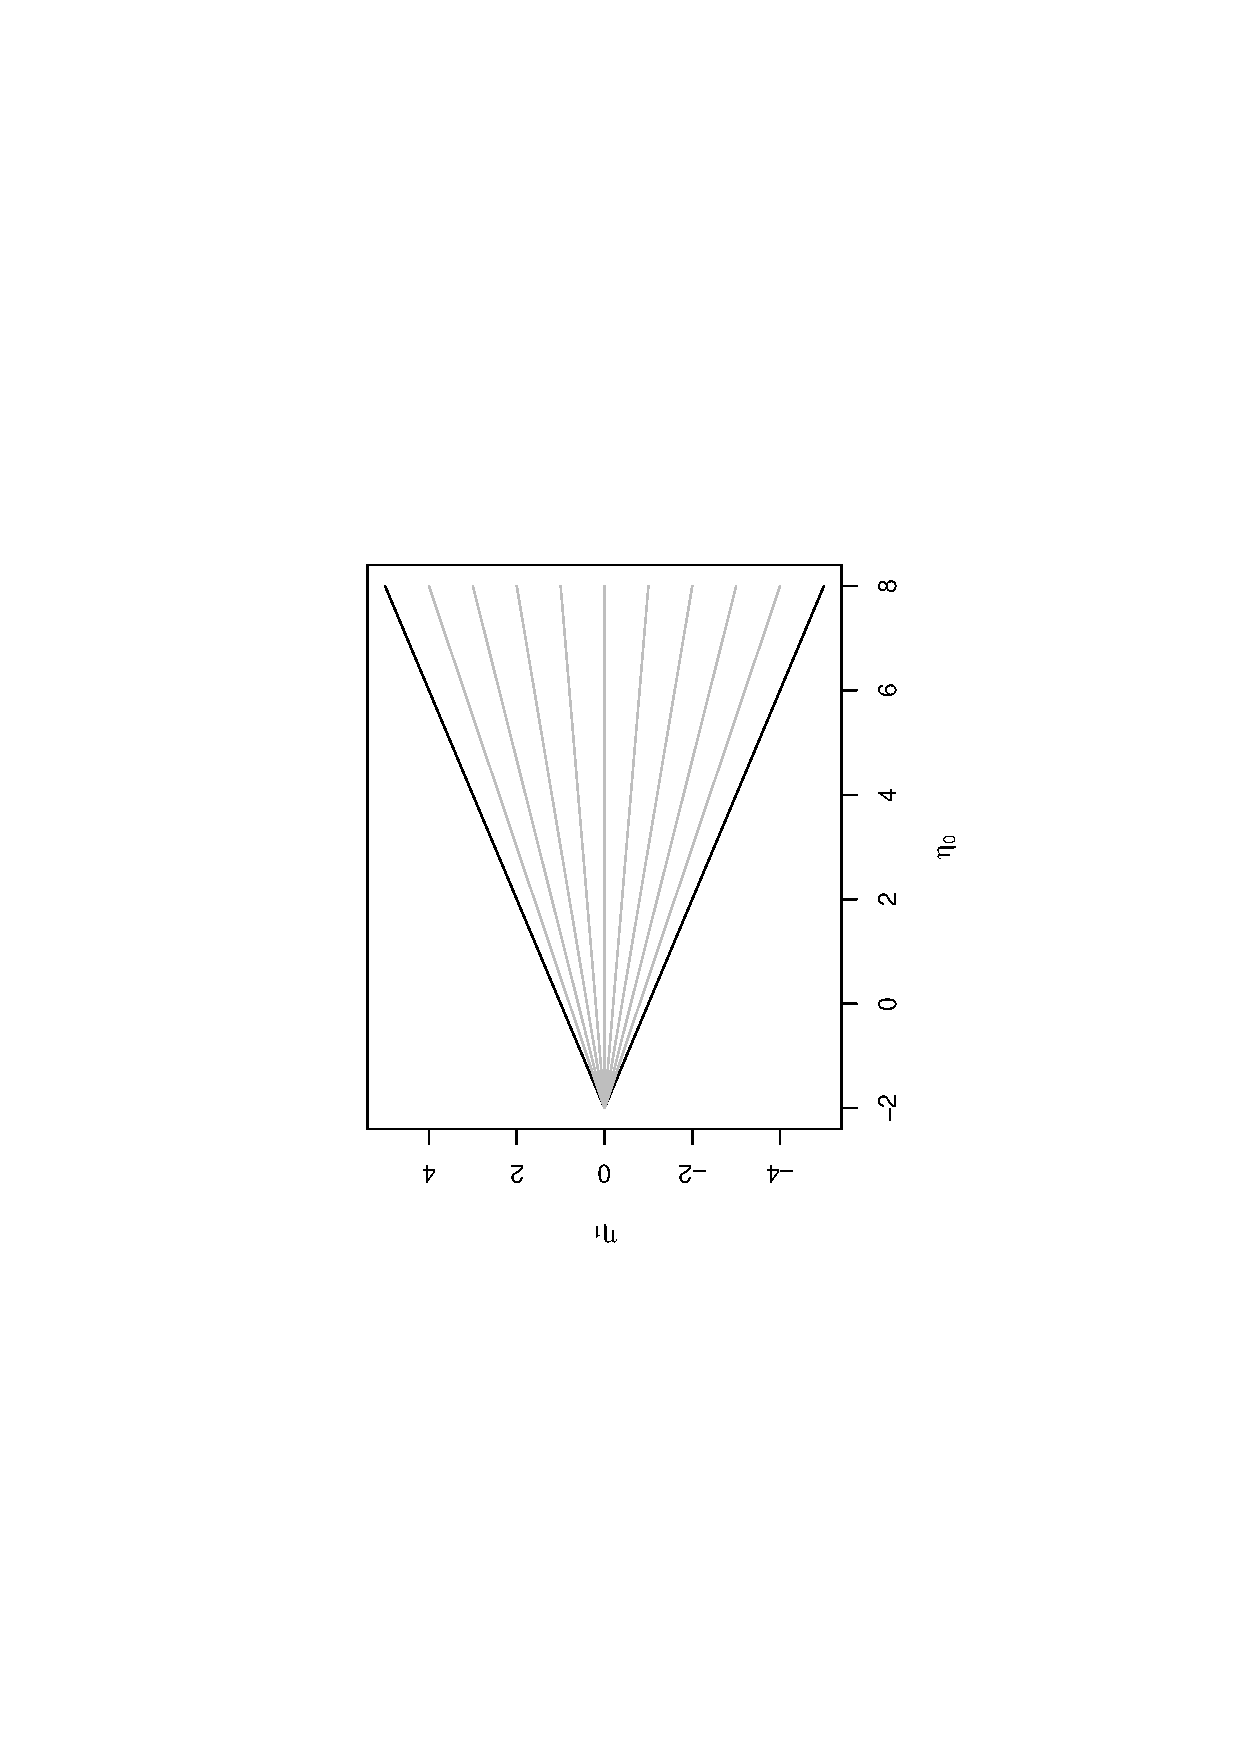
\includegraphics[trim = 80mm 45mm 80mm 60mm, clip, width=0.7\textwidth]{R/boatshape-domain}
\caption[Bounds for the domain of $\eta_0$ and $\eta_1$ for the Beta-Binomial model,
with rays of constant expectation for $y_c = \{0.1,0.2,\ldots,0.9\}$.]%
{Bounds for the domain of $\eta_0$ and $\eta_1$ for the Beta-Binomial model (black),
with rays of constant expectation for $y_c = \{0.1,0.2,\ldots,0.9\}$ (grey).}
\label{fig:boatshape-domain}
\end{figure}

As we wrote in Section~\ref{sec:concluding-outlook},
$\eta_1$ cannot have the convenient property of being equal to
the expectation of the mean sample statistic $\ttau(\x)$ (here, $s/n$),
as was the case for $y$.%
\footnote{For $\yz$, it holds that $\yz = \E\big[\E[\ttau(\x) \mid \psi] \mid \nz, \yz\big]$,
as mentioned in Section~\ref{sec:regularconjugates}.}
However, from \eqref{eq:trafotony} we can derive that coordinates $(\eta_0,\eta_1) \in \Eta$ satifying
\begin{align}
\label{eq:raysofconstantexpectation}
\eta_1 = f(\eta_0) &= (\eta_0 + 2)(y_c - \frac{1}{2}) 
\end{align}
will have a constant expectation $y_c$.
The domain $\Eta$, and these \emph{rays of constant expectation} emanating from the coordinate $(-2,0)$,
are depicted in Figure~\ref{fig:boatshape-domain}.







%
